\documentclass[12pt, a4paper]{article}

\usepackage[slovene, english]{babel}
\usepackage[utf8]{inputenc}
\usepackage{amsmath, amsfonts}
\usepackage{url}
\usepackage{graphicx}
%\usepackage{tikz}
\usepackage{textpos}
\usepackage{wrapfig}
\usepackage{amsthm}
%\usepackage{enumitem}
\usepackage{physics}

\newtheorem{izrek}{Izrek}
\newtheorem{trditev}{Trditev}
\newtheorem{lema}{Lema}
\newtheorem{definicija}{Definicija}
\newtheorem{pos}{Posledica}
\newtheorem{zgled}{Zgled}
\newtheorem{naloga}{Naloga}

\newcommand{\R}{\mathbb R}
\newcommand{\N}{\mathbb N}
\newcommand{\Z}{\mathbb Z}
\newcommand{\C}{\mathbb C}
\newcommand{\Q}{\mathbb Q}

\renewcommand{\mod}{\operatorname{mod}}

\title{Funkcije več spremenljivk}
\author{Karmen Zupančič, Žiga Flajs, Jakob Svetina \\ Mentor: Žan Hafner Petrovski}
\date{
\includegraphics[width = 6cm]{logo_MaRS2017.png}}

\begin{document}
\selectlanguage{slovene}
\maketitle

\begin{abstract}
V članku spoznamo funkcije več spremenljivk in se previdno dotaknemo pomembnih tem iz analize. Začnemo z grafi funkcij dveh spremenljivk, potem pa se osredotočimo na polarne in sferične koordinate, s pomočjo katerih pridemo do sicer že znanih rezultatov, ampak na nov in širše uporaben način. Zaključimo pa s posebno funkcijo, ki predstavlja razširitev fakultete na pozitivna realna števila.
\end{abstract}

\section{Uvod}
Vsak naj bi poznal funkciije ene spremenljivke, saj se jih obravnava že v osnovni šoli. Kdor potem nadaljuje šolanje, se z njimi še bolje spozna, redki pa se spoznajo s funkcijami več spremenljivk. Grafi takih funkcij so dosti težje predstavljivi kot grafi funkcij ene spremenljivke, ki jih lahko dokaj enostavno upodobimo na ravnini. Čim več spremenljivk nastopa v prostoru iz katerega slikamo, tem bolj zapleteni so njihovi grafi, zapletenost pa v tem primeru vodi do večje svobode in nam odpira vrata do bolj abstraktnih idej.

\section{Funkcije dveh spremenljivk}

\begin{definicija}
\textbf{Funkcija dveh neodvisnih spremenljivk} je predpis, ki vsakemu paru $(x,y)$ iz podmnožice ravnine predpiše natančno določeno realno število.
Velja torej: 
$$f : \mathbb{R}^2 \rightarrow \mathbb{R}$$
$$f:(x,y) \mapsto z=f(x,y).$$

\end{definicija}

Realno število, ki je prirejeno spremenljivkam v trorazsežnem prostoru pomeni višino nad točko. Upodabljamo lahko le funkcije z do dvema spremenljivkama, za funkcije treh ali večih spemenljivk pa je upodabljanje njihovega grafa na ljudem predstavljiv način nemogoče. Za razliko od funkcij z eno spremenljivko upodabljamo grafe lepih funkcij dveh spremenljivk s ploskvijo, ki ima enačbo $z-f(x,y)=0$. Spoznali smo nekaj grafov preprostih funkcij, ogledali pa smo si tudi primere zahtevnejših funkcij dveh spremenljivk.

\begin{zgled}
Funkcija $f(x,y)=x^2+y^2$ Graf funkcije je dvorazsežni objekt v trorazsežnem prostoru.
\end{zgled}

\begin{figure}[h!]
\centering
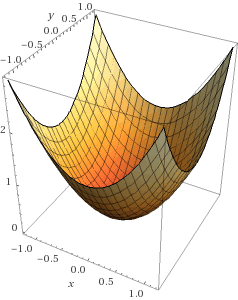
\includegraphics{slika_funkcije.PNG}
\caption{Graf funkcije f(x,y)}
\end{figure}

\newpage
\begin{zgled}
Primer zahtevnejše funkcije $g(x,y)=x^2 sin(x)y^3$ 
\end{zgled}

\begin{figure}[h!]
\centering
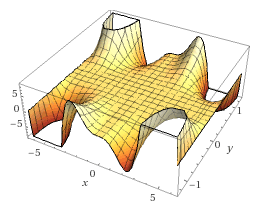
\includegraphics{funkcija_2.PNG}
\caption{Graf funkcije g(x,y)}
\end{figure}

\section{Volumen krogle}

Izračunali smo tudi volumen krogle z različnimi metodami. Začnimo s to, ki smo jo spoznali že v gimnaziji, kasneje pa bomo do iste formule prišli še na drug način. 

\begin{zgled} 
Izračun prostornine vrtenine, ki nastane z vrtenjem grafa funkcije $f(x)=\sqrt{(1-x^2)}$. Graf te funkcije nad zaprtim intervalom $[-1,1]$ je ravno zgornja polovica enotstke krožnice, zato je rotacijsko telo enotska sfera, integral pa predstavlja volumen krogle.

Uporabimo formulo iz gimnazije in rezultat hitro sledi:
$$V=\pi \int_{a}^b{f(x)}^2\mathrm{d} x$$
$$V=\pi \int_{-1}^1{{\sqrt{(1-x^2)}}}^2\mathrm{d} x=\pi(x-\frac{x^3}{3})\big|_{-1}^1= \pi (1-\frac{1}{3})-\pi (-1+\frac{1}{3})$$
$$V=\frac{4}{3}\pi$$
\end{zgled}


\section{Izrek o zamenjavi spremenljivk v integralu}
Najprej se bomo seznanili s primerom zamenjave ene spremenljivke potem pa bomo spoznali še zamenjavo dveh in treh spremenljivk v integralu.
\\
Naj bo $f$ zvezna na $[a,b]$ in $\phi$ zvezno odvedljiva funkcija, ki interval $[\alpha,\beta]$ preslika bijektivno na interval $[a,b]$ tako, da je  $\phi(\alpha)=a$ in $\phi(\beta)=b$. Tedaj je

$$\int_{a}^bf(x)\mathrm{d} x=\int_{\alpha}^{\beta}f(\phi(t))\phi'(t)\mathrm{d} t$$

Na podoben način lahko zamenjamo več spremenljivk. 
\begin{izrek}
Naj bo $U \subset \mathbb{R}^n$ odprta množica z volumnom $\neq 0$ in $g:U \rightarrow \mathbb{R}^n$ dovolj lepa preslikava. Naj bo $\big | \det Dg(t) \big |\neq 0$ za vse $t \in U$ in omejena na $U$. Predpostavimo, da ima $g(U)$ volumen. Za vsako integrabilno funkcijo $f:g(U) \rightarrow \mathbb{R}$ velja:

$$\int_{g(U)}^{}f(x) \mathrm{d} V=\int_{U}^{}f(g(t)) \big |\det Dg(t) \big | \mathrm{d} V$$
\end{izrek}

%%%%%%%%%%%%%%%%%%%%%%%%%%%%%%%%%%%%%%
\section{Računanje determinante reda 2 in 3}

Oglejmo si, kako izračunati determinanto reda 2 in 3. Navedene so eksplicitne formule za njihov izračun.

\[
\begin{vmatrix}
    a& b  \\
   c &d \\
\end{vmatrix}
=ad-bc
\]

\[
\begin{vmatrix}
 a&b&c\\
 d&e&f\\
 g&h&i\\
\end{vmatrix}
=a\begin{vmatrix}
e&f\\
h&i\\
\end{vmatrix}-b\begin{vmatrix}
d&f\\
g&i\\
\end{vmatrix}+c\begin{vmatrix}
d&e\\
g&h\\
\end{vmatrix}
\]



%%%%%%%%%%%%%%%%%%%%%%%%%%%%%%%%%%%%%%

\section{Polarne koordinate}
Polarni koordinatni sistem je ravninski koordinatni sistem, ki je osnova za sferični koordinatni sistem. Točko v polarnem koordinatnem sistemu podamo z dvema polarnima koordinatama:
\begin{itemize}
\item $r$ - razdalja od točke do koordinatnega izhodišča (dolžina vektorja $\vec{r}$)
\item $\phi$ - kot med $x$-osjo in smerjo vektorja $\vec{r}$
\end{itemize}

Da iz polarnih koordinat dobimo koordinati kartezičnega koordinatnega sistema $x$ in $y$, uporabimo preslikavo $g:[ 0,\infty)    [0,2\pi]  \rightarrow  \mathbb{R}^2$ s sledečim predpisom:
$$g(r,\phi) = (r \cos \phi, r \sin \phi)$$

Kartezični koordinati torej z $r$ in $\phi$ izrazimo takole:
\begin{itemize}
\item $x=r \cos \phi$
\item $y=r \sin \phi$
\end{itemize}

\begin{figure}[h!]
\centering
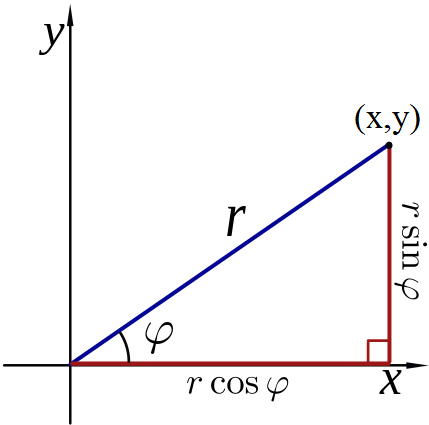
\includegraphics[width=.3\textwidth]{polarne_koordinate.png}
\caption{Grafični prikaz prejšnje izražave}
\end{figure}



\section{Sferične koordinate}

Sferični ali krogelni koordinatni sistem je krivočrtni sistem koordinat v trirazsežnem prostoru, s pomočjo katerega enolično določimo lego točk na sferi ali sferoidu. Za določanje lege točke v prostoru vedno potrebujemo tri koordinate. Pri sfernem koordinatnem sistemu uporabljamo sferične koordinate:
\begin{itemize}
\item $r$ - razdalja od točke do koordinatnega izhodišča (dolžina vektorja $\vec{r}$)
\item $\phi$ - kot med $x$-osjo in smerjo pravokotne projekcije vektorja $\vec{r}$ na $xy$-ravnino
\item $\theta$ - kot med ravnino $x$-$y$ in vektorjem $\vec{r}$
\end{itemize}

Da iz polarnih koordinat dobimo koordinate kartezičnega koordinatnega sistema $x$, $y$ in $z$, uporabimo preslikavo $g:  [ 0,\infty)    [0,2\pi]    [-\frac{\pi}{2}]  \rightarrow \mathbb{R}^3 $ s predpisom:
$$g(r,\phi, \theta) = (r \cos \phi \cos \theta, r \sin \phi \cos \theta, r \sin \theta)$$

Dobimo koordinate:
\begin{itemize}
\item $x=r \sin \phi \cos \theta$
\item $y=r \cos \phi  \cos \theta $
\item $z=r \sin \theta$
\end{itemize}

(manjka še slika kot pri polarnih koordinatah)


\section{Parcialni odvod}

%parcialne odvode moramo spoznati, da lahko uporabimo zgornji izrek

Denimo, da je $f : \mathbb{R}^2 \rightarrow \mathbb{R} $ je funkcija dveh spremenljivk.

Parcialna odvoda po $x$ in po $y$ funkcije $f$ v točki $(a, b)$ definiramo (podobno kot odvod pri funkciji ene spremenljivke) kot limiti ustreznih parcialnih diferenčnih kvocientov (pri pogoju, da ti dve limiti obstajata):
$$
f_x(a, b)= \frac{\partial f}{\partial x}(a, b) = \lim_{h\to\infty} \frac{f(a+h, b)}{h}
$$
$$
f_y(a, b)= \frac{\partial f}{\partial y}(a, b) = \lim_{k\to\infty} \frac{f(a, b+k)}{k}
$$

Parcialna odvoda torej izračunamo tako, da odvajamo funkcijo na $x$ oziroma na $y$ po znanih pravilih za odvajanje funkcij ene spremenljivke, pri čemer smatramo drugo spremenljivko za konstanto.

\begin{zgled}

Za funkcijo $f(x, y)= x^2+xy+y^2$ je $\frac{\partial f}{\partial x}= 2x+y+y^2$ in $\frac{\partial f}{\partial y}= 2y+x+x^2$.

\end{zgled}

\section{Jacobijeva matrika}
Jacobijeva matrika preslikave $g: \mathbb{R}^2 \rightarrow \mathbb{R}^2$ oziroma $g: \mathbb{R}^3 \rightarrow \mathbb{R}^3$ je matrika, ki jo sestavljajo parcialni odvodi prvega reda.

Matrika reda 2 ima obliko:
$$
Jg(x_1,x_2)=
\begin{bmatrix}
\frac{\partial g_1}{\partial x_1} & \frac{\partial g_2}{\partial x_1}  \\
\frac{\partial g_1}{\partial x_2} & \frac{\partial _2}{\partial x_2} 
\end{bmatrix}
$$

Matrika reda 3 ima obliko:
$$
Jg(x_1,x_2,x_3)=
\begin{bmatrix}
\frac{\partial g_1}{\partial x_1}  & \frac{\partial g_2}{\partial x_1}  & \frac{\partial g_3}{\partial x_1}  \\
\frac{\partial g_1}{\partial x_2}  & \frac{\partial g_2}{\partial x_2}  & \frac{\partial g_3}{\partial x_2}  \\
\frac{\partial g_1}{\partial x_3}  & \frac{\partial g_2}{\partial x_3}  & \frac{\partial g_3}{\partial x_3} 
\end{bmatrix}
$$



\section{Ploščina kroga in volumen krogle}

\begin{naloga}
S pomočjo polarnih koordinat in parcialnih odvodov izpelji formulo za računanje ploščine kroga. \\
\emph
{Najprej izračunamo parcialne odvode polarnih koordinat:}

\begin{itemize}
\item $\frac{\partial x}{\partial r}= \cos \phi$
\item $\frac{\partial x}{\partial \phi}= r  (-\sin \phi)$
\item $\frac{\partial y}{\partial r}= \sin \phi$
\item $\frac{\partial y}{\partial \phi}= r  \cos \phi$ \\
\end{itemize}
\emph
{Parcialne odvode izračunamo, vstavimo v Jacobijevo matriko in izračunamo njeno determinanto.}
\\
\begin{center}
 {
$\det (Jg)(r,\phi)=$ \large $ \begin{vmatrix} \frac{\partial x}{\partial r}  &  \frac{\partial x}{\partial \phi}  \\  \frac{\partial y}{\partial r}  &  \frac{\partial y}{\partial \phi}  \end{vmatrix} $ $=$ \normalsize $\begin{vmatrix} \cos \phi & -r \sin \phi \\ \sin \phi & r \cos \phi \end{vmatrix} $  $= r$
}
\end{center}

\emph
{Dobimo determinanto diferenciala preslikave $g$, ki jo vstavimo v dvojni integral:}
\begin{eqnarray*}
\int^{2\pi}_{0} \int^{R}_{0}   \begin{vmatrix} \det Dg \end{vmatrix}  \mathrm{d} r \mathrm{d}\phi &=&  \int^{2\pi}_{0} \int^{R}_{0}  r \mathrm{d} r \mathrm{d}\phi \\
 &=&  \int^{2\pi}_{0} \frac{r^2}{2} \big|^{R}_{0} \mathrm{d}\phi \\
 &=&  \int^{2\pi}_{0} \frac{R^2}{2} \mathrm{d}\phi \\
 &=&  \frac{R^2}{2} \phi  \big|^{2\pi}_{0} \\
 &=&  \frac{R^2}{2} 2\pi \\
 &=&  \pi R^2
\end{eqnarray*}

\emph
{Ugotovimo, da smo dobili formulo za računanje površine kroga:}
$$
S=\pi r^2
$$
\end{naloga}


\begin{naloga}
S pomočjo sferičnih koordinat in parcialnih odvodov izpelji formulo za volumen krogle.

\emph{Podobno kot prej izračunamo parcialne odvode in jih vpišemo v matriko, s katero izračunamo determinanto:}
\\
\begin{center}
$ \det (Jg)(r,\phi, \theta)$ $=$  \\ $=$ \large  $\begin{vmatrix} \frac{\partial x}{\partial r}  &  \frac{\partial x}{\partial \phi} &  \frac{\partial x}{\partial z} \\  \frac{\partial y}{\partial r}  &  \frac{\partial y}{\partial \phi} &  \frac{\partial x}{\partial z} \\ \frac{\partial \theta}{\partial r}  &  \frac{\partial \theta}{\partial \phi} &  \frac{\partial \theta}{\partial z} \end{vmatrix} $ 
$=$  \normalsize $ \begin{vmatrix} \cos \phi  \cos \theta & \sin \phi  \cos \theta & \sin \theta \\ r \sin \phi  \cos \theta  & r \cos \phi  \cos \theta  & 0 \\ -r \cos \phi  \sin \theta  & -r \sin \phi  \sin \theta  & r \cos \theta \\ \end{vmatrix} $  $=$ $r^2 \cos \theta $
\end{center}

\emph{Determinanto vstavimo v trojni integral:} \\

\begin{eqnarray*}
\int^{\frac {\pi}{2}}_{- \frac {\pi}{2}} \int^{2\pi}_{0} \int^{R}_{0}  \big | \det Dg \big | \mathrm{d} r \mathrm{d}\phi \mathrm{d}\theta  &=&  \int^{\frac {\pi}{2}}_{- \frac {\pi}{2}} \int^{2\pi}_{0} \int^{R}_{0}   r^2 \cos \theta   \mathrm{d} r \mathrm{d}\phi \mathrm{d}\theta  \\
 &=&  \int^{\frac {\pi}{2}}_{- \frac {\pi}{2}} \int^{2\pi}_{0} \cos \theta \frac {r^3}{3} \big |^{R}_{0} \mathrm{d}\phi \mathrm{d}\theta  \\
 &=&  \int^{\frac {\pi}{2}}_{- \frac {\pi}{2}} \int^{2\pi}_{0} \cos \theta \frac {R^3}{3} \mathrm{d}\phi \mathrm{d}\theta  \\
 &=&  \int^{\frac {\pi}{2}}_{- \frac {\pi}{2}} \cos \theta \frac {R^3}{3} \big |^{2 \pi}_{0} \mathrm{d} \theta  \\
 &=&  \int^{\frac {\pi}{2}}_{- \frac {\pi}{2}} \frac {2 \pi R^3}{3} \cos \theta \mathrm{d} \theta  \\
 &=&  \frac {2 \pi R^3}{3} \sin \theta \big |^{\frac {\pi}{2}}_{-\frac {\pi}{2}}  \\
 &=&  (2) \frac {2 \pi R^3}{3}  \\
 &=&  \frac {4 \pi R^3}{3}  \\
\end{eqnarray*}

\emph
{Ugotovimo, da smo dobili formulo za računanje volumna krogle:}
$$
V=\frac{4\pi r^3}{3}
$$
\end{naloga}

%%%%%%%%%%%

\section{Eulerjeva $\Gamma $-funkcija}

Pri delu s funkcijami z več spemenljivkami smo spoznali tudi funkcijo gama. Prvi je funkcijo zapisal Leonhard Euler leta 1729, ko je pisal pismo svojemu prijatelju matematiku. Odvisna je le od ene spremenljivke in slika pozitivna realna števila $\mathbb{R}^+$ v realna $\mathbb{R} $. Funkcija je zanimiva, saj če v njo vstavimo celo pozitivno število $n$, potem lahko izračunamo fakulteto števila $n-1$.
\begin{definicija}
Funkcija gama je za $t>0, t\in\mathbb{R}$, definirana kot:
\[ \Gamma (t) = \int^{\infty}_{0} x^{t-1} e^{-x} \mathrm{d} x \]
\end{definicija}

\begin{izrek} 
\label{izrek:enacbazagamo}
Za izračun $n!$ s funkcijo $ \Gamma (t)$ se uporablja enačba:
\[ \Gamma (t) = (t - 1) \Gamma (t-1) \] 
\end{izrek}


Če izrek uporabimo za vrednost $ \Gamma (t-1) $, tako da  $$ \Gamma (t-1) = (t-1) \Gamma (t-2),$$ in postopek ponovimo za vsako nasljedno manjšo vrednost $t$,
potem velja: 
\begin{izrek}
\[ \Gamma (t) = (t-1)! \].
\end{izrek}
%, quote izrek,enačba

Do zapisanega smo prišli z integriranjem funkcije po načinu per partes. Ker se enačbe za per partes na začetku nismo spomnili, smo jo enostavno izpeljali iz pravila za odvajanje produkta funkcij.
\begin{eqnarray*}
 (f \cdot g)' = f' \cdot g + f \cdot g' \\
(f \cdot g)' - f' \cdot g =  f \cdot g' \\
(f \cdot g)' - f' \cdot g =  f \cdot g' ~~ \Big| \cdot \int \\
fg - \int f'g = \int fg' 
\end{eqnarray*}

Če se resno lotimo dokazovanja, da za naravno število $t$ velja $ \Gamma (t) = (t-1)!$, kar smo tudi storili, bodo enačbe funkcije izgledale tako:
\begin{eqnarray*} 
\Gamma (t) = \int^{\infty}_{0} e^{-x} x^{t-1} \mathrm{d} x &=& x^{t-1} e^{-x} \Big|^{\infty}_{0} + \int^{\infty}_{0} e^{-x} x^{t-2} (t-1) \mathrm{d} x \\
&=&  (t-1) \cdot \int^{\infty}_{0} e^{-x} x^{t-2} \mathrm{d} x \\
&=& (t-1) \Big( e^{-x} x^{t-2} \Big|^{\infty}_{0} + (t-2) \int^{\infty}_{0} e^{-x} x^{t-3} \mathrm{d} x \Big) \\
&=& (t-1)(t-2) \int^{\infty}_{0} e^{-x} x^{t-3} \mathrm{d} x = \ldots = (t-1)! ~ , 
\end{eqnarray*}
saj je $ \lim_{x \to \infty} \dfrac{x^{t-1}}{e^x} = 0 $. 

Izbrane vrednosti funkcije, pri katerih je spremenljivka $t \in \mathbb{R^{+}}$, so izračunane v sledeči tabeli.

\begin{center}
\begin{tabular}{| c || c | c | c | c | c | c |}
\hline
$t$ & $\frac{1}{2}$ & 1 & $\frac{3}{2}$ & 2 & $\frac{5}{2}$ & 3 \\
\hline
$\Gamma (t)$ & $\sqrt{\pi}$ & 1 & $\frac{\sqrt{\pi}}{2}$ & 1 & $\frac{3 \sqrt{\pi}}{4}$ & 2 \\
\hline
\end{tabular}
\end{center}

\begin{figure}[h!]
\centering
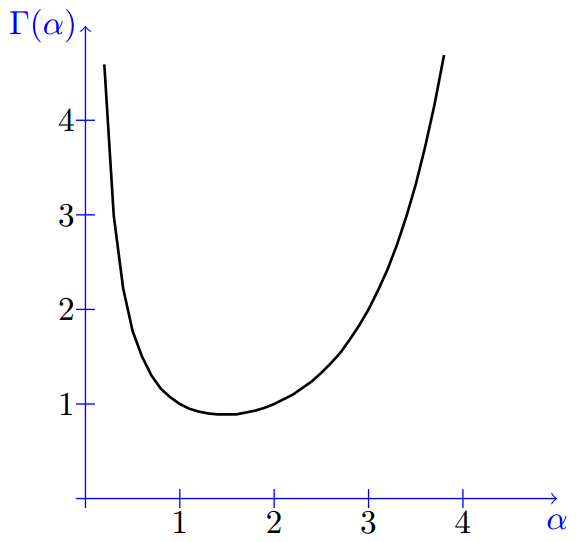
\includegraphics[width=0.45\textwidth]{gama.png}
\caption{Graf funkcije $ \Gamma (t) $}
\end{figure}

Ko se spremenljivka $t$ bliža neskončnosti, gre tudi $ \Gamma (t)$ proti neskončnosti. Podobno se zgodi, ko se $t$ bliža vrednosti 0:
\begin{itemize}

\item $ \lim_{t \to \infty} \Gamma (t)= \infty $
\item $ \lim_{t \to 0} \Gamma (t)= \infty $
\end{itemize}

Opisana funkcija nam je v pomoč pri izražanju nekaterih integralov. Mi smo naredili naslednji primer:
\[ \int^{\infty}_{0} x^{\frac{1}{3}} e^{-x}\mathrm{d} x = \frac{\Gamma (\frac{4}{3})}{3^{\frac{4}{3}}}. \]














%http://www.fmf.uni-lj.si/~hladnik/Analiza/ParcialniOdvodi.pdf



\end{document}